% This is samplepaper.tex, a sample chapter demonstrating the
% LLNCS macro package for Springer Computer Science proceedings;
% Version 2.21 of 2022/01/12
%
\bibliography{VAD/FILES/Reference}
\bibliographystyle{splncs04}
\documentclass[runningheads]{llncs}
%
\usepackage[T1]{fontenc}
% T1 fonts will be used to generate the final print and online PDFs,
% so please use T1 fonts in your manuscript whenever possible.
% Other font encondings may result in incorrect characters.

\usepackage{graphicx}
\usepackage{amsfonts}
\usepackage{booktabs}
\usepackage{siunitx}
\usepackage{subfig}
\usepackage{indentfirst}
\usepackage{multirow}
\usepackage{multicol}
\usepackage[font=small,labelfont=bf]{caption}
\usepackage{orcidlink}

\usepackage{xcolor}
\hypersetup{
    colorlinks,
    linkcolor={red!50!black},
    citecolor={blue!50!black},
    urlcolor={black}
}
%%%%%
% Used for displaying a sample figure. If possible, figure files should
% be included in EPS format.
%
% If you use the hyperref package, please uncomment the following two lines
% to display URLs in blue roman font according to Springer's eBook style:
%\usepackage{color}
%\renewcommand\UrlFont{\color{blue}\rmfamily}

\begin{document}
 
\title{Multi-layer Embedded Video Anomaly Detection using Attention Driven Recurrence}

% Multilayer embedded Video Anomaly Detection and Classification using Attention Driven Spatio-Temporal Features
% Deep Learning based Video Anomaly Detection and Classification with Efficient Spacio-Temporal Attention and Recurrence

%\titlerunning{Abbreviated paper title}

% If the paper title is too long for the running head, you can set
% an abbreviated paper title here

% \author{
% Ummay Maria Muna \orcidlink{https://orcid.org/0009-0002-0746-8661} \and
% Shanta Biswas \orcidlink{https://orcid.org/0009-0009-1147-0095} \and
% Syed Abu Ammar Muhammad Zarif \orcidlink{https://orcid.org/0009-0005-2417-8289} \and
% Philip Jefferson Deori \orcidlink{https://orcid.org/0009-0002-4280-0236} \and
% Tauseef Tajwar \orcidlink{https://orcid.org/0009-0006-9163-0172} \and
% Swakkhar Shatabda \orcidlink{https://orcid.org/0000-0003-0669-072X}
% }

\author{
First Author \orcidlink{https://orcid.org/} \and
Second Author \orcidlink{https://orcid.org/} \and
Third Author \orcidlink{https://orcid.org/} \and
Fourth Author \orcidlink{https://orcid.org/}
}


% \authorrunning{U. Muna et al.}
\authorrunning{author1 et al.}
% First names are abbreviated in the running head.
% If there are more than two authors, 'et al.' is used.
%
% \institute{United International University, Dhaka, Bangladesh \\
% \email{\{umuna201429,sbiswas201418,szarif202009,pdeori202111\}@bscse.uiu.ac.bd, \ \{tauseef,swakkhar\}@cse.uiu.ac.bd}}

\institute{Institute
\email{lncs@springer.com}\\
\url{http://www.springer.com/gp/computer-science/lncs}
}

\maketitle

\begin{abstract}
Automated Video Anomaly Detection (VAD) is a challenging task due to its context-dependent and sporadic nature. Recent deep learning advancements offer promising solutions. In this paper, we propose a spatio-temporal analysis-based video anomaly detection method where we address challenges such as lengthy videos and anomaly sparsity in an anomalous video by segmenting and labeling anomalous parts, integrating a sliding window system, and employing multilevel embedding creation techniques. We enhance feature representation using customized ResNet50 and introduce the parameter-efficient SRU++ recurrent model with an attention mechanism for the efficient processing of embedding sequences. Additionally, a cluster-based weighing mechanism was also incorporated to further enhance the prediction capability. Extensive evaluation utilizing different approaches on the UCF Crime dataset demonstrates our approach's superior performance compared to state-of-the-art methods, making it suitable for real-world surveillance scenarios.

\keywords{Video Anomaly Detection \and Deep Learning \and Simple Recurrent Neural Networks \and Attention Mechanism \and Spatio-Temporal Feature Analysis \and Segmentation \and Multilevel Embedding \and Clustering}
\end{abstract}

\section{Introduction}

Surveillance systems are well integrated into most public and private places for activity monitoring and record-keeping, and thus ensuring safety and maintaining judicial accountability naturally becomes a high priority in all societies and organizations. Surveillance systems tend to produce data at high rates, and scanning through hours of footage to find an incident that has already occurred requires intense manual labor and does not make addressing the incident a relatively fast job, leading to a need to automate surveillance monitoring. Video anomaly detection involves a stream of data \cite{sertis}. When translated to real life, anomalous data would be a person breaking a law or regulation, which should stand in contrast to non-anomalous data, which is a person who is compliant with societal norms, laws, and regulations. Nevertheless, achieving accurate anomaly detection poses a daunting challenge, given the diverse and sometimes subtle nature of abnormal events that involve ambiguity. They are often contextual and subjective, varying depending on the environment, which poses challenges for the VAD task. In addition, the lengthy duration of videos is associated with the fact that the most anomalous events occupy a small portion of the video. \cite{Multi-contextual} \cite{Memory-Token} \cite{zhao2022exploiting}

Recent advancements in deep learning have demonstrated remarkable success in the field of video anomaly detection. The reconstruction-based technique has been a widely used unsupervised approach where only normal video is used for training and to learn the normal pattern, thus generating errors when fed with abnormal patterns. However,  traditional reconstruction or next frame prediction based methods solely analyze a single frame, ignoring the crucial temporal connection between the frames. On the other hand, spatio-temporal information processing from all categories of data is another frequently used supervised technique where both the spatial features of the frames and the temporal relationship among the frames are taken into consideration. However, most existing methodologies encounter challenges in learning and distinguishing events and their multidimensional patterns, primarily  due to the extended duration of anomalous videos containing only sporadic instances of  actual anomalies.\cite{challenges} Therefore, proper anomalous data should be fed in order to create a better anomaly learner. The VAD process involves extensive calculations; therefore, parallel calculations could make faster predictions, and high recurrence could enable the approach to capture long term dependencies in sequential temporal data.

In this paper, we present a comprehensive approach to anti-social video anomaly detection and multi-class classification. It recognizes the challenges posed by the large duration of video data, like the UCF crime dataset and the infrequent nature of anomalous events within the videos. Our segmentation approach divides and labels the anomalous parts into fixed-length manageable segments, which makes the model better distinguishable from all the categories. Additionally, to facilitate real time anomaly detection, a sliding window system was integrated to traverse the video gradually rather than at once. We incorporated spatio-temporal feature analysis techniques, which will assist the model in understanding the motion evolution of objects. Moreover, for the purpose of meaningful feature representation, a multilevel feature extraction technique was applied using the powerful ResNet50. Afterwards, a lightweight and parameter efficient recurrent model, Simple Recurrent Unit Plus Plus (SRU++), integrated with an attention mechanism was effectively utilized to make the technique highly recurrent and parallelizable, making it suitable for processing large volumes of feature sequences. In addition to further improving accuracy, we employ clustering techniques to partition the spatio-temporal features of training data into distinct clusters for all classes, subsequently introducing a novel weighing mechanism upon clustering at the test phase. Through comprehensive evaluation and testing, our approach achieved excellent performance on UCF Crime dataset and outperformed many state-of-the-art methods. Figure 1 shows the overall architecture of this paper. 

\noindent
The overview of the contribution of this paper as follows:

\begin{enumerate}

\item A perfect segmentation and label representing the true anomaly and non anomaly datasets was generated from the UCF crime dataset, which contains a great portion of the non-anomaly activity of an anomalous video. A sliding window was traversed throughout the video for real world anomaly detection.

\item A multi-level feature extraction module was adopted to fuse both raw and abstract level video features. The ResNet50 model was incorporated to generate complex hierarchical feature representations.

\item We introduced the efficient use of highly recursive SRU++ augmented with an attention layer in the computer vision domain for VAD to process the temporal relationships of the sequential video feature embeddings. This architecture facilitated the training of the embeddings alongside their corresponding labels.

\item Additional clustering and weight assignment mechanisms were integrated to further enhance the classification accuracy.

\end{enumerate}

\begin{figure}
\centering
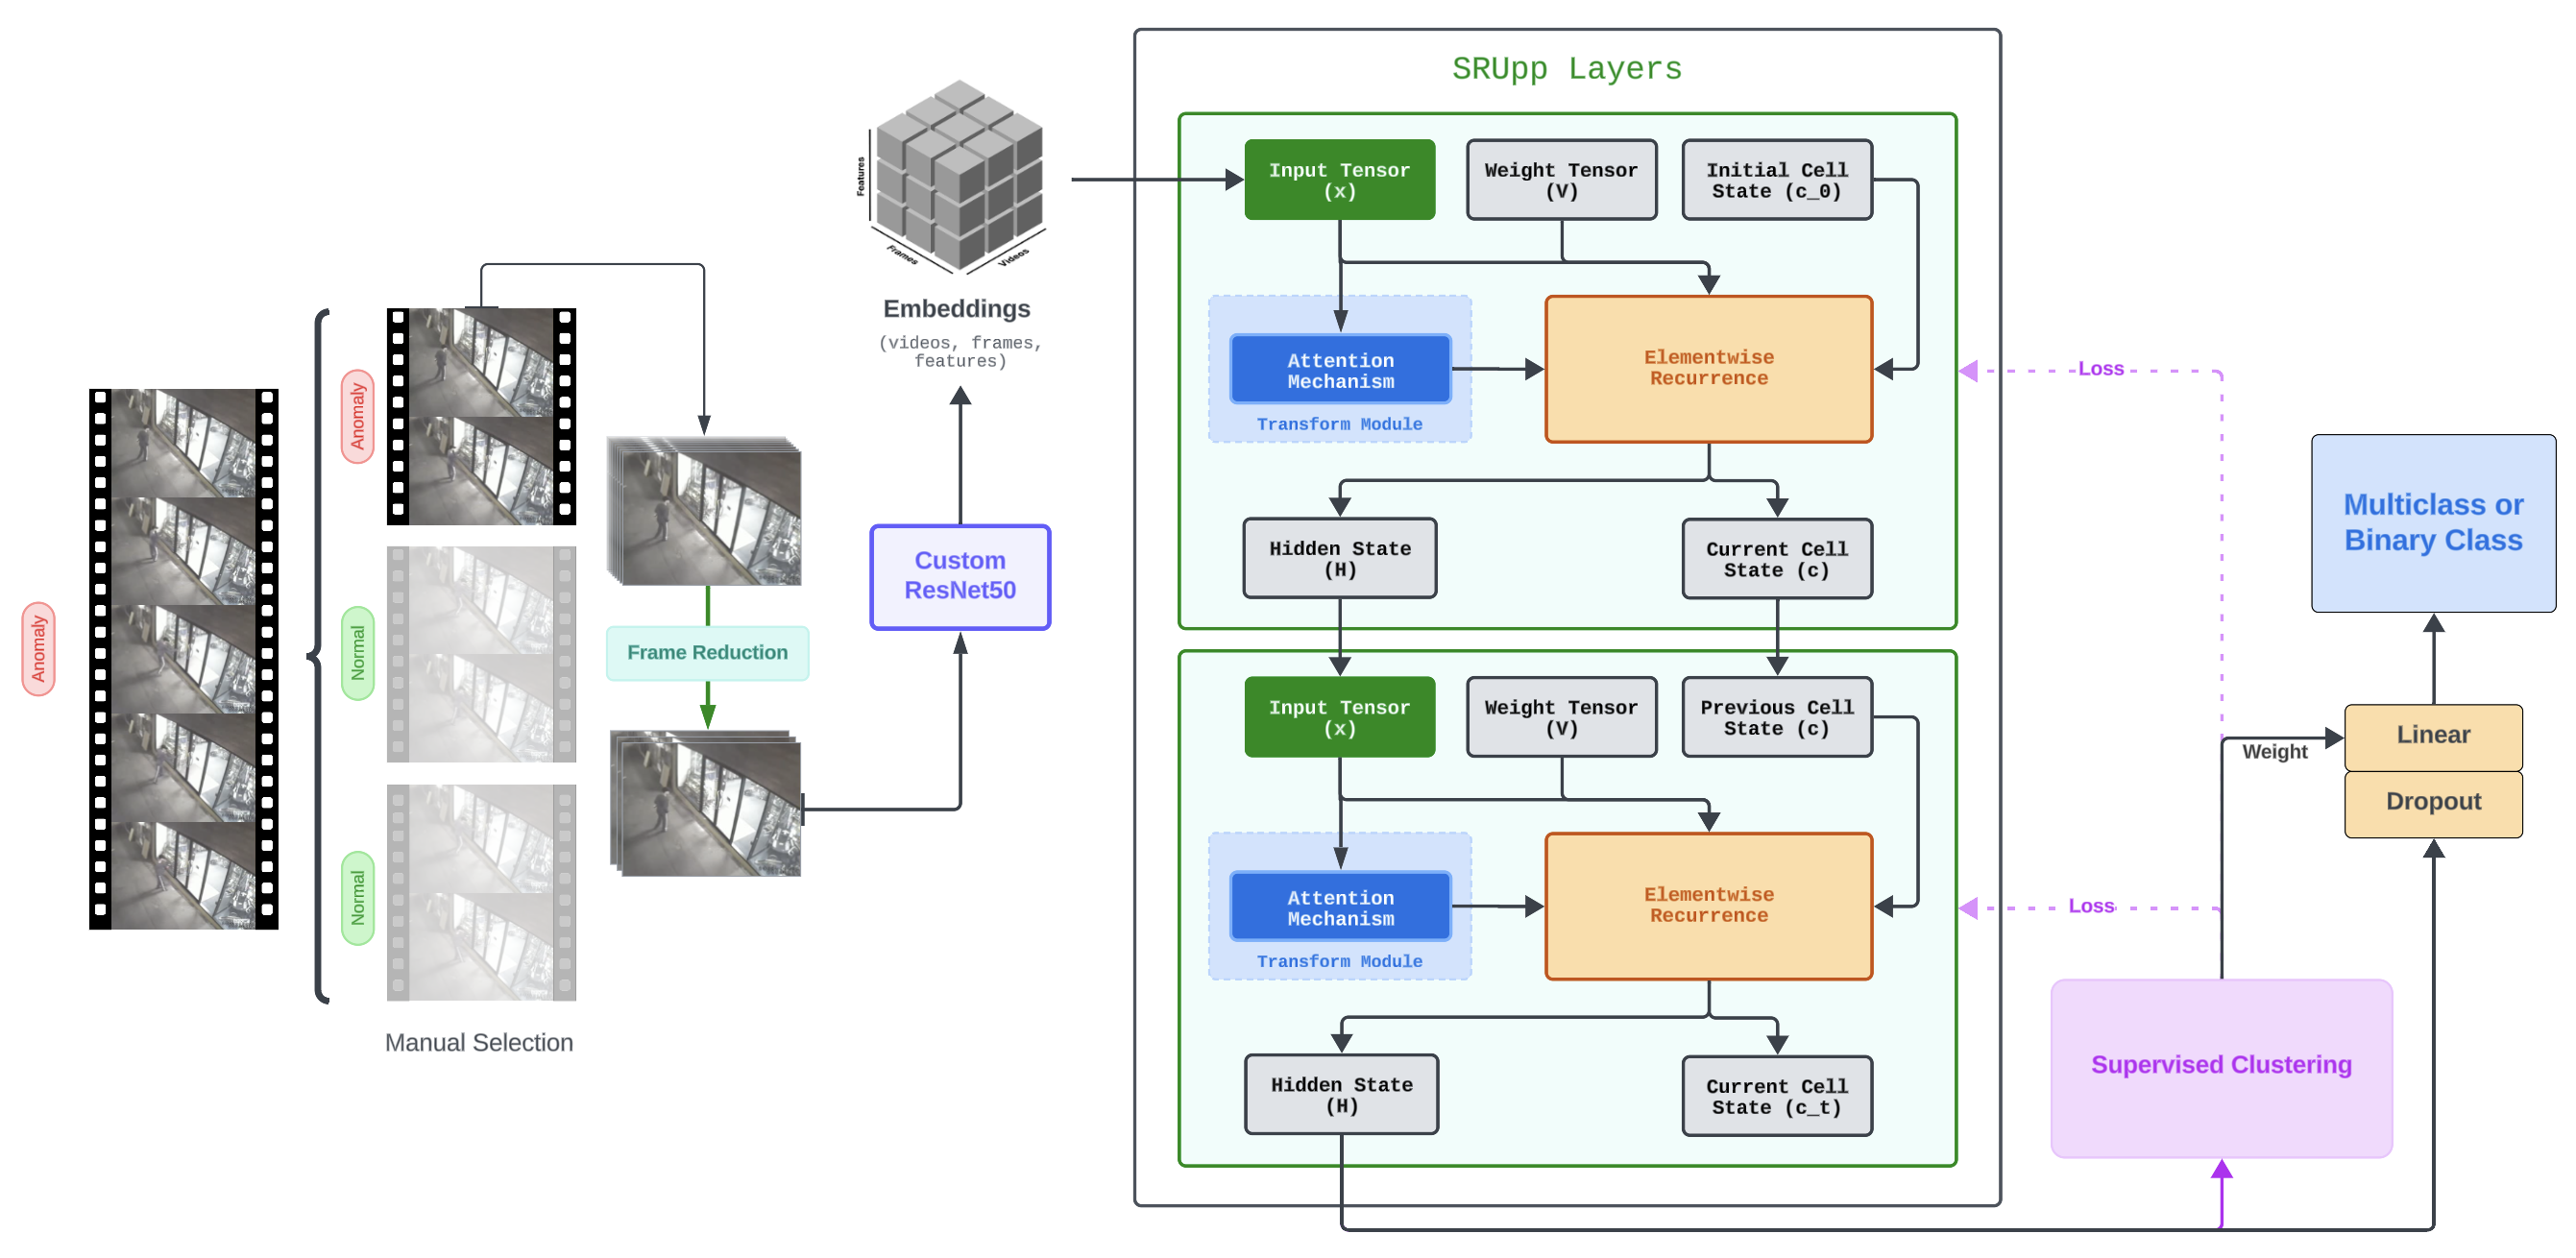
\includegraphics[width=0.9\textwidth]{VAD/FIGURES/reduced_pipeline_final.png}
\caption{\textbf{Overview of the proposed pipeline:} A lengthy video (the figure depicts an anomaly video) is first  segmented into several short clips, which are later manually labeled. Each clip is then subjected to a frame reduction procedure and processed by a custom ResNet50 architecture to generate feature embeddings. These embeddings are then utilized to train an SRU++ model for anomaly classification. Additionally, during training, data exhibiting similar patterns is clustered to facilitate a weighting mechanism that enhances classification accuracy.} \label{fig1}
\end{figure}

\section{Literature Review}

\subsection{Spatio-temporal feature extraction based methods}
Spatial-temporal analysis has been a broadly used supervised VAD technique and many researchers have shown promising results on different datasets. Swathikiran et al. \cite{sudhakaran} proposed a deep neural network that employs a CNN to extract features, which are then aggregated using a variant of LSTM. The proposed model produces promising results. \cite{petrocchi} adapted the deep learning technique to extract contextual, spatial and motion features from videos. Moreover, YOLOv4 was used as the object detection model, while spatial and motion information were extracted using ResNet-50. On a similar note, \cite{vosta2022cnn} designed a CNN based violence detection technique associated with ResNet-50 for feature extraction, which is then followed by a particular schema of RNN, ConvLSTM for the purpose of violence detection. Zahid et al. \cite{islam2021efficient} achieved the same task of violence detection by implementing Separable Convolutional LSTM and MobileNet when tested on the RWF-2000 dataset. \cite{zhang2019temporal} addressed VAD by studying the evolution regularity of appearance and motion through the spatial and temporal correlations within adjacent frames using the spatio-temporal long short-term memory in order to understand spatial appearances and temporal variations.\cite{zhao2022exploiting} employs Multiple Instance Learning (MIL) for weakly supervised anomaly detection. They proposed Inner Bag Loss (IBL) for MIL considering the lowest anomaly instance score and the highest score in each individual bag. Maryam et al. \cite{qasim2023video} employed a CNN followed by a SRU based automated system that is capable of identifying anomalies within videos by analyzing spatial and temporal features. \cite{shao2023video} extracted temporal representations from the input video, where the correlation between positive and negative samples is studied. 
\subsection{Reconstruction and Prediction based methods}
Throughout the years, great strides have been made in video anomaly detection using reconstruction based and prediction based methods. \cite{end2end} proposed an end-to-end framework combining prediction based and reconstruction based models that also utilizes reconstruction loss as spatial attention and showed good performance.\cite{multivit} Using self-supervisory simultaneous prediction with three different contextual prediction streams and optical flow, a model was designed to learn normality patterns and further improve performance with optical flow information. Consistency-Aware High-Level Feature Extractor (CAFE)\cite{cafe} uses a student-teacher architecture to prioritize high level semantics, and a consistency-aware scheme allows low-level differences to be ignored temporarily. Further integration of generic frameworks allowed low level information to be considered as well. Prior Knowledge Guided Network (PKG-Net)\cite{pkgnet} designed a feature based framework by using an auto-encoder network for frame prediction and a block-wise knowledge distillation technique that allows both large scale details from feature inconsistency maps and fine scale details from prediction error to be considered during anomaly detection. STATE\cite{state} takes advantage of pretrained object detection models to extract object patches from video frames and generate spatio-temporal information, then passes through a convolutional auto-encoder for motion and pixel-level reconstruction and learning spatio-temporal attention. \cite{ma} utilized a temporal augmented network based approach that allows motion aware features to be considered along with spatial and temporal information for anomaly detection. An MIL ranking model using attention blocks was used to differentiate between anomalous and non-anomalous video segments by comparing their scores.
\subsection{Transformer and Attention applied based Methods}
The transformer based approach is another heightening approach for VAD task, since it helps to extract out the most important part of the data. \cite{Multi-contextual} employed ViT in pixel level prediction,  utilizing three contextual prediction streams for frame reconstruction, including whole, masked, and partial situation. Additionally, they integrated flow reconstruction to  enhance abnormal event detection. \cite{attention-anomaly} utilized Videoswin transformer followed by attention layers to  generate frame-level anomaly scores, capturing the temporal long and short range dependencies. \cite{contrastive} incorporate GCN with a discriminative function to filter normal segments and derived normal features from anomalous videos using a contrastive attention module. Their approach utilizes three distinct loss functions for attention weight consistency and segment-level classification.. Hannah et al. \cite{Cross-attention} proposed TIAN for video interpolation, introducing a cross similarity to aggregate input image features globally, which were eventually refined by an image attention module. Another study \cite{Memory-Token} introduced the Memory-Token Transformer (MMT) that encodes the spatio-temporal features by 3D convolution and fused the semantic tokens of the videos. \cite{multi-view} employed frameworks with an attention schemes to localize anomalies effectively. One uses the memory addressing module, while the next one introduced a novel loss function for multiple instance learning. \cite{SwinAnomaly} extracted the video features using Swin Transformer alongside a GAN based 3D auto-encoder to predict the future frame using a 2D decoder. They have also incorporated real time VAD mechanism. \cite{TransCNN} built an end-to-end hybrid framework combined with CNN and Vision Transformers. The CNN model extracts the spatial features and the transformer learns the temporal relationships.

\section{Methodology}

\subsection{Datasets}
The UCF-Crime dataset is a large-scale dataset containing 1900 long and un-trimmed real-world surveillance videos. It has 13 class realistic anomalies videos such as abuse, arrest, arson, assault, road accident, burglary, explosion, fighting, robbery, shooting, stealing, shoplifting, and vandalism, which are very impactful to society and should be detected as soon as they occur. The dataset additionally includes another class, which contains 950 surveillance videos with normal activities. However, the "arrest" and "shoplifting" classes were excluded due to their potential anomalies and confusion, as "arresting" is typically not considered an anomaly and "shoplifting" is covert and context-dependent, which may confuse the model. The motivation for using this dataset is that the paper is solely intended to address all the illegal and anti-social activities that cause harm to society.

\subsection{Preprocessing}
The paper went through an extensive preprocessing technique since the videos of the UCF dataset are lengthy while the anomalous portion stayed for a very short period of time. To mitigate these issues, the videos within the dataset were thoroughly segmented into fixed-length chunks, and the repeated and redundant segments were removed. Subsequently, the true label was assigned to all 12 classes. Due to the fixed-length segmentation, multiple anomalous segments were generated from a single anomalous video containing the different patterns. Therefore, a total of 3500 segmented videos were generated, representing true anomalous  and non anomalous activities. However, the data distribution was uneven, so it exhibited class imbalance. Among them, half of the videos belong to the normal class, and the other half belong to all other classes. Afterwards, the dataset was augmented by doubling its size through horizontal flipping of all normal and anomalous videos. Therefore, the total number of video data points increased to 7,000. The dataset was split into two portions, which are the train set and the test set, at an 80:20 ratio.

\subsection{Multilevel Feature Fusion and Derivation Module}
Videos are represented in high dimensional numerical form as they contain information about the height, width and channels of each frame and processing a video in its raw numerical form demands high computational costs with many redundancies especially in video anomaly detection. Therefore, the frames are encoded into a lower-dimensional vector representation called embedding while maintaining meaningful semantic information; so that the model can effectively capture the semantic and visual features of the frames sequentially. However, a good feature extractor is required to retrieve the underlying features and patterns. The paper uses customized ResNet-50 \cite{he2015deep}, known for its robust feature extraction capabilities due to its residual connections. While the ResNet model extracts complex image features robustly, the deep level of convolutional layered architecture may overlook the local patterns in the frames and extract more abstract features. This paper uses a customized ResNet50 where the model will extract and combine both high and low level features to maintain meaningful multilevel fused feature representation. It takes the $j^{th}$ frame of the video $f_{ij}$ sequentially. While being processed by the layers of the model, the content extracted by the middle layer (L3) is stored as a more localized and raw level feature representation. Likewise, the overall global features from the last layer (L5) are treated as global and abstract features. Both of the feature spaces are then fused together by taking the mean value. 

\begin{figure}
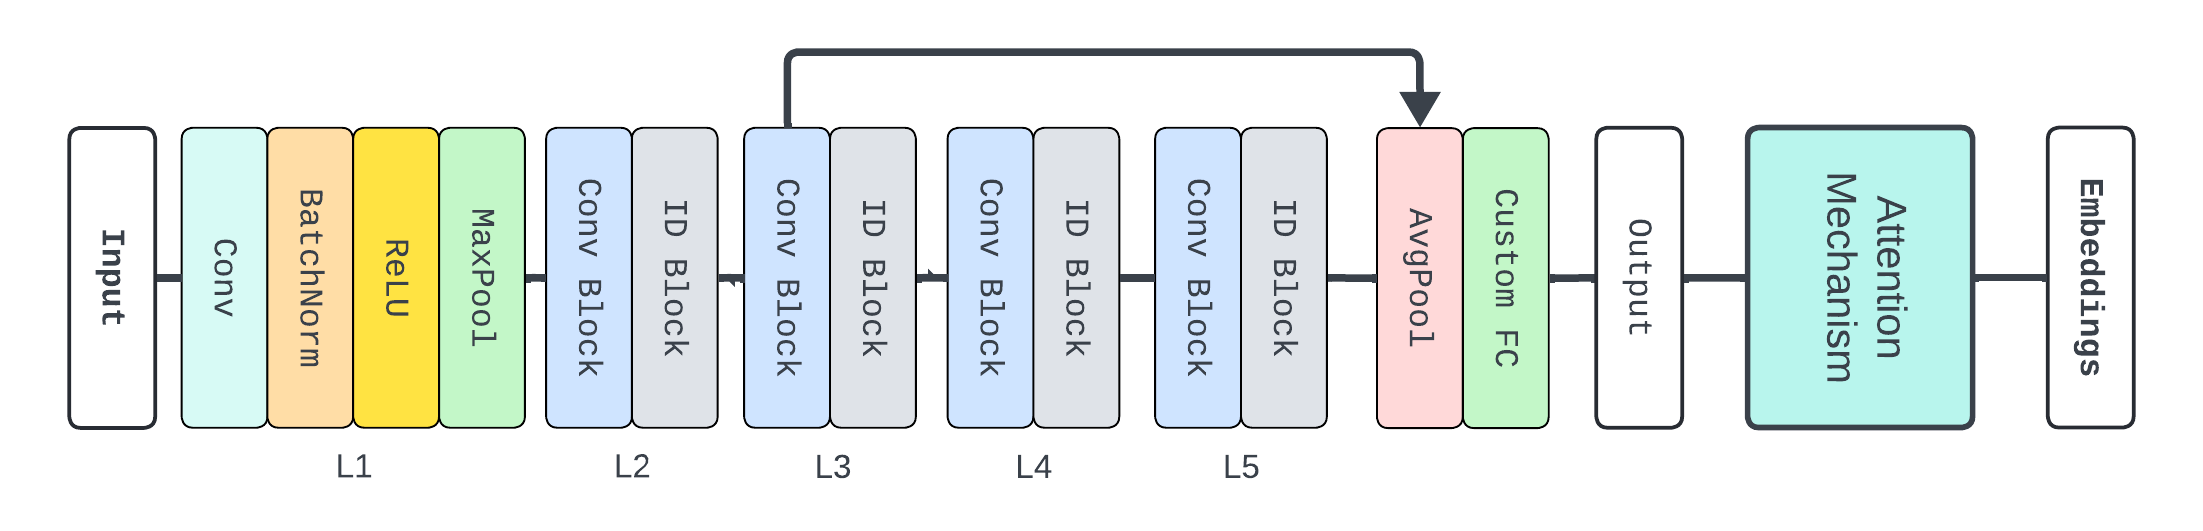
\includegraphics[width=\textwidth]{VAD/FIGURES/custom-resnet50.png}
\caption{Multilevel Feature Extraction with Custom ResNet-50} \label{fig2}
\end{figure}

\noindent Afterwards, the extracted feature goes through an attention mechanism to further prioritize the important and meaningful sequences. The attention mechanism consists of two linear layers followed by two activation functions $tanh$ and $softmax$ respectively to generate the weight values which are later multiplied by the extracted features. The final attended embedding is then prepared to feed into the sequential model later.

\subsection{Attended Simple Recurrent Network Module}

A simple recurrent neural network  \cite{lei2018simple} is a light and parameter efficient recurrent neural network that has a high recurrence parallelized gate calculation mechanism with CUDA level optimization. This unlocks the full parallel processing power of a GPU that helps the model capturing the long range sequential data and compute across the hidden dimensions at time steps. Furthermore, the inclusion of highway connections facilitates direct information propagation across frame embeddings, aiding in understanding the temporal evolution of visual features. This paper has employed the extended version of the SRU which integrates attention mechanism in every $n{th}$ layer called SRU++ \cite{lei2021attention} to enhance the model's ability to capture crucial aspects of long-range sequences. \\

The attended SRU applies the elementwise recurrence to calculate the four gates: hidden state $h_t$, forget gates $f_t$, reset gates $r_t$ and the current cell state $c_t$ shown in equation equation 1-4.
\begin{equation}
f_t = \sigma(W_fx_t + v_f \odot c_{t-1} + b_f) 
\end{equation}
\begin{equation}
c_t = f_t \odot c_{t-1} + (1-f_t) \odot (Wx_t)
\end{equation}
\begin{equation}
r_t = \sigma (W_rx_t + v_r \odot c_{t-1} +b_r)
\end{equation}
\begin{equation}
h_t = r_t \odot c_t + (1 - r_t) \odot x_t 
\end{equation}
\begin{figure}
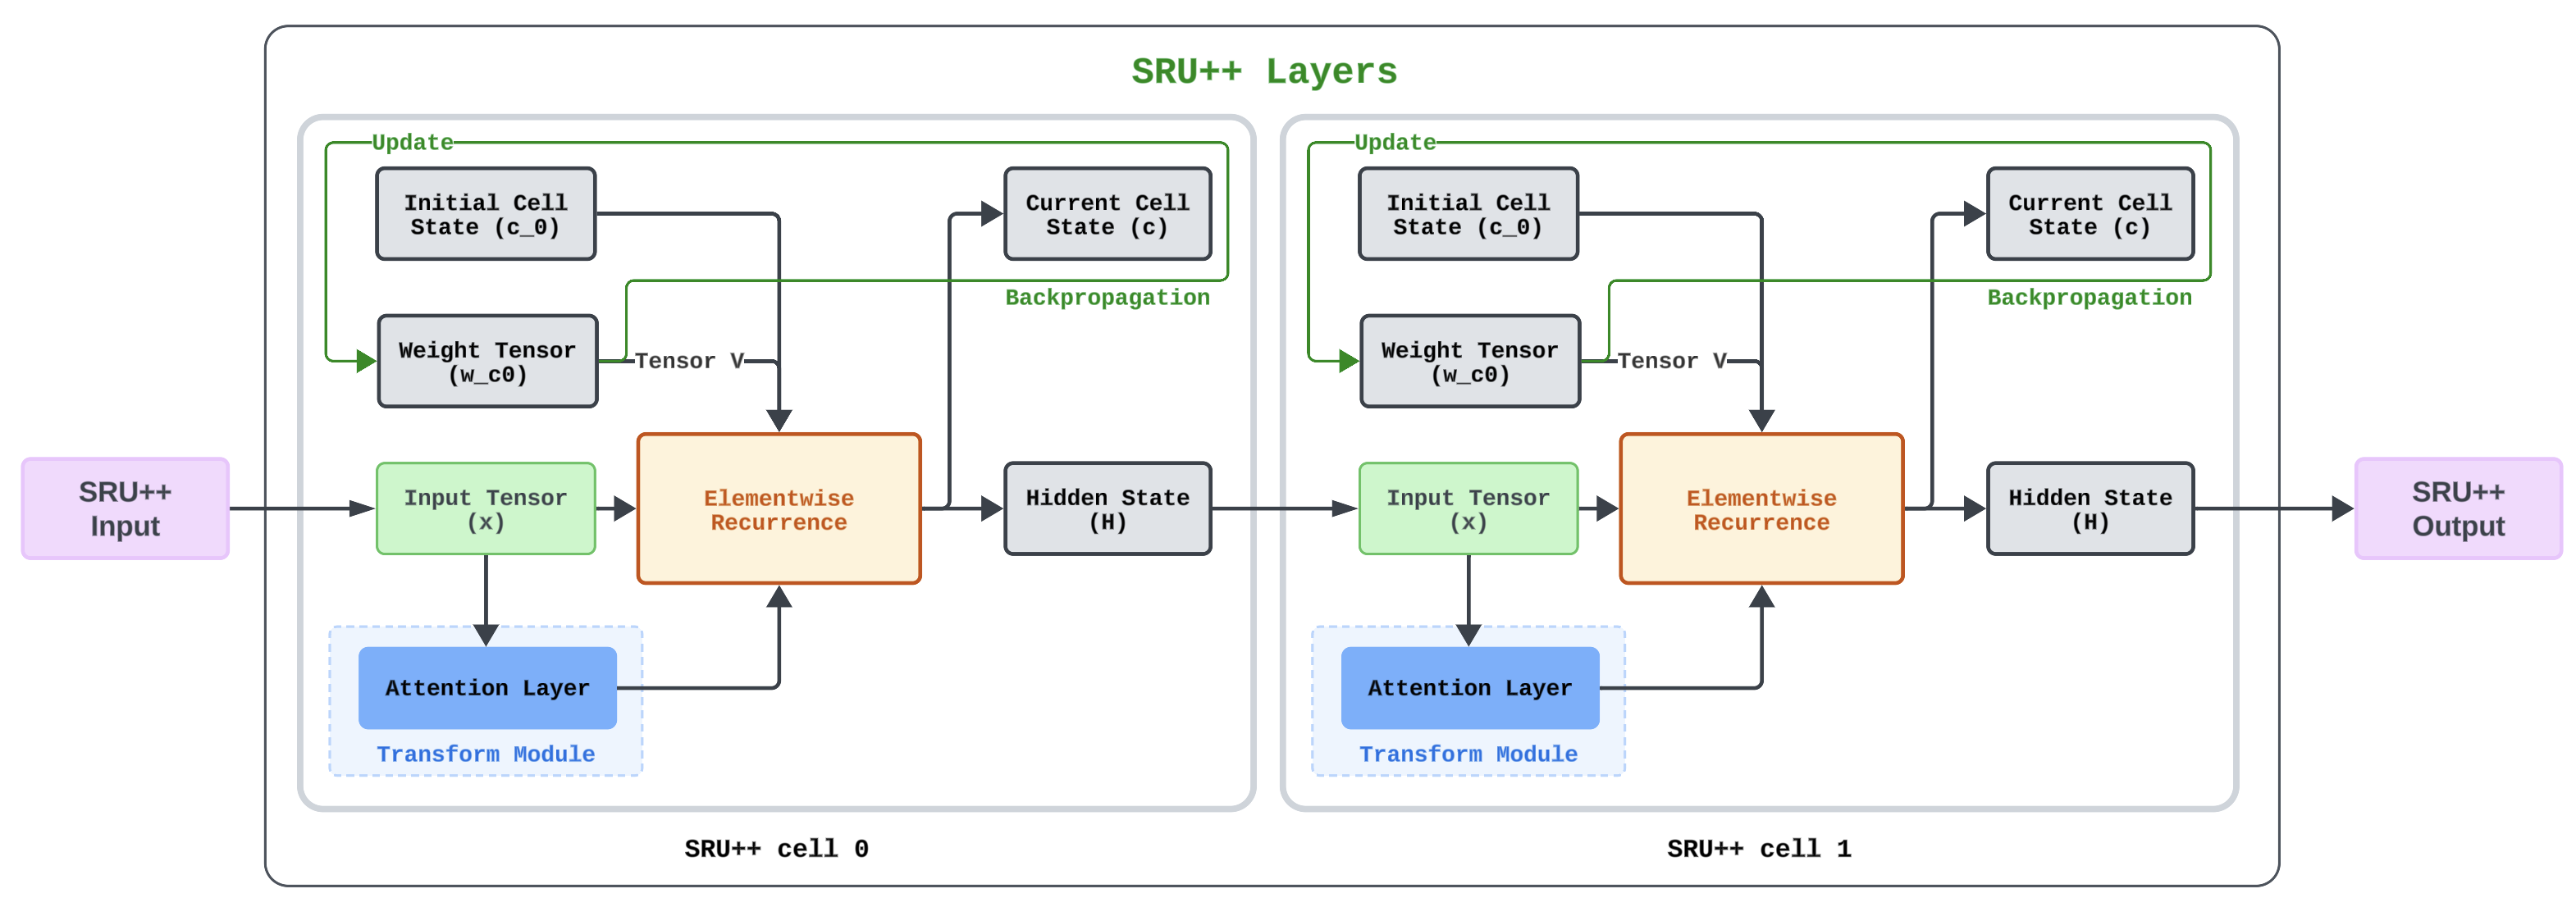
\includegraphics[width=\textwidth]{VAD/FIGURES/srupp-details-transparent.png}
\caption{Two Layered Attended Simple Recurrent Unit} \label{fig3}
\end{figure}\\

\noindent
\textbf{i) Simple recurrent Unit}\\

Attended SRU consists of stacked attention based simple recurrent cells that are connected sequentially. Each cell incorporates a self-attention mechanism to capture long-range dependencies in an input sequence. This mechanism is useful for anomaly detection in videos because detecting anomalies in a video requires understanding the long-range frame dependencies. In an attention-based simple recurrent unit mechanism, we feed an input sequence $x_{(l, b, f_i)}$, it generates temporal feature $t_{(l,b,f_o)}$, where $l$, $b$, $f_i$, and $f_o$ denote sequence length, batch size, input feature vector dimension and output feature dimension respectively. Finally using $t_{(l,b, f_o)}$, the model classifies a video.\\

In the attended SRU, the first input $x_{(l,b,f_i)}$ is projected to $x'_{(l,b,f'_i)}$, where $f’$ is the new projected feature dimension of shape $2048$. This linear transformation enriches feature representation, which helps the attention mechanism in effectively distinguishing important aspects, enhancing the model’s learning capacity. After projecting, we feed the $x'_{(l,b,f'_i)}$ into the model which has two SRU++ cell connected sequentially. The projected input propagates from first cell $s_0$ to final cell $s_1$ that generates the temporal feature $t_{(l,b,f_o)}$ which is expressed in equation ($6$).
\begin{equation}
t_{(l,b,f_o)} = SRU(x'_{(l,b,f'_i)})
\end{equation}

The temporal feature $t_{(l,b,f_0)}$ is processed by a dropout layer followed by a linear layer that predicts the class probability $P$ of the corresponding classes. If the dropout layer is $\Delta_{dropout}$, the linear layer is $^{1024, 2}\!\mathcal{L}$ and $C_n$ represents all the classes; with equation $(6)$, the model can predict the class probability $P(C_n)$, where $n$ is the class number.

\begin{equation}
P(C_n) = \ ^{1024, 2}\!\mathcal{L}((\Delta_{dropout}(t_{(l,b,f_o)})))\\
\end{equation}\\

\vspace{-5mm}
\noindent
\textbf{ii) Attended simple recurrent cell}\\

The model consists of two cells that are connected sequentially. Each cell generates a hidden state $h_t$ which propagates to the input of the next cell, a cell state $c_t$. At first, a multiheaded attention mechanism is applied to the projected input  $x'_{(l,b,f'_i)}$ and creates attention output $U_{(lb, f_on)}$. Each cell has a weight matrix $V_{(2\times f_o)}$s through backpropagation and a cell state $c_0$, This cell state contains information that propagates through both layers. With the projected input $x'_{(l,b,f'_i)}$, attended output of input matrix $U_{(lb, f_on)}$, weight matrix  $V_{(2\times f_o)}$ and cell state $c_0$, the attended simple recurrent cell calculates all the gate values by elementwise recurrence technique using CUDA level optimization. The output of the elementwise recurrence is hidden state $h_t$ and cell state $c_t$, which is then propagated to the next layer. \\

\noindent
\textbf{iii) Multihead Attention}\\

A multihead attention mechanism applies attention to the projected input $x’_{(l, b, f'_i)}$ . It consists of eight attention heads which allows the module to attend to eight different aspects, capturing broader and more diverse relationships within the frame sequence. Query $Q$, key $K$ and value $V$ are extracted from the projected input $x’_{(l, b, f'_i)}$ from two linear layers $^{1024, 1024}\! \mathcal{L}_Q$ and $^{1024, 2048}\!\mathcal{L}_{KV}$. Equations $(7)$ and $(8)$ depict how $Q, K$ and $V$ is extracted.

\begin{equation}
Q = \ ^{1024, 1024}\mathcal{L}_Q(x’_{(l, b, f'_i)}) = W_Q x’_{(l, b, f'_i)}
\end{equation}

\begin{equation}
K, V = \ ^{1024, 2048}\mathcal{L}_{KV}(x’_{(l, b, f'_i)}) 
= W_K x’_{(l, b, f'_i)} , W_V x’_{(l, b, f'_i)}
\end{equation}

In the next step, eight attention heads are created from the $Q$, $K$ and $V$ with their weight matrices $W_Q$, $W_K$ and $W_V$. Each head contains query $Q_i$, key $K_i$ and value $V_i$ where $i$ is the attention head index. For each head, we scale the query matrix $Q$ by a factor of $\frac{1}{\sqrt{d_k}}$, where $d_k$ is the feature dimention of key $K$ matrix which is later multiplied by the transposed key matrix $K^T$ to calculate the unnormalized attention score. A softmax activation function and dropout is applied to this unnormalized attention score followed by performing matrix multiplication with value matrix $V$, which is the attention output $U$.
\begin{equation}
U = \Delta_{dropout}(softmax(\frac{QK^T}{\sqrt{d_k}}))V
\end{equation}


\subsection{Feature Cluster Weighing module}
Additionally, our core methodology effectively weighted the classification score upon a clustering technique to further improve the accuracy. We employed the supervised clustering technique using the spatio-temporal feature derived from the SRU++ module. The cluster was formulated by providing the class label at each iteration. While forming the clusters $\{l_1, \ \ldots, \ l_{12}\}$ , cluster centers were also generated and refined at each step; therefore, the final cluster centers $\{c_1, \ \ldots, \ c_{12}\}$ were derived. At the test phase, for each datapoint the features were extracted using the trained module and cosine similarity is shown in equation 10, between the cluster centers and the data points was calculated. The cluster with the highest cosine similarity was taken into consideration. Therefore, when a  test data point aligns with a cluster, we assign a weight w to that particular class label prediction score p[i] given in equation 11, followed by a normalization. This weight is proportional to the  confidence level that the test data point belongs to the correct class. By leveraging this technique, we prioritize their influence on the final classification decision. If a predicted cluster for a datapoint is denoted by $d_i$ and its predicted cluster is denoted by $c_i$ then,

\begin{equation}
  \text{Cosine Similarity}(\mathbf{a}, \mathbf{b}) = \frac{\mathbf{a} \cdot \mathbf{b}}{\|\mathbf{a}\| \|\mathbf{b}\|} \label{eq:cosine_similarity}  \\
\end{equation}

\begin{equation}
  i = \text{sim}(d_j, c_i)_{\text{max}} \label{eq:cluster}  ,
  \quad p[i] = p[i] \times w \label{eq:weight}  
\end{equation}\\

\section{Experimental Evaluations}

\subsection{Implementation Details}

In this study, for feature extraction, 100 frames are sampled uniformly and resized into $224 \times 224 \times 3$ of height, width and channel respectively from a 10 second video segment recorded at 30fps. The feature extraction module. Frames are passed sequentially through the feature extractor module, which returns a $1024$ size frame embedding by fusing multilevel features from L3 and L5. Lastly, an attention module, consisting of two linear layers and two activation functions ($tanh$ and $softmax$) is applied to the mean feature vector. At the end of the phase, we get a $(7000, 100, 1024)$-shaped feature embedding, representing the total videos, total frames and embedding size of the frames. \\

After splitting the dataset into train test, the training subset  is fed into the SRU++ model sequentially in $b_n = 8$ batches. The SRU++ model is configured with two cells, empirically selected to be optimal. The model processes a $1024$-dimensional feature vector, generating a hidden state $h_t$ and cell state $c_t$ where $c_t$ is discarded due to its internal usage in recurrent gate calculation. A dropout layer of $0.2$, followed by a fully connected layer is applied in the hidden state $h_t$ that classifies the video into different classes. 8 attention heads are used with a scaling factor of $\frac{1}{\sqrt{h_d}}$ where $h_d$ is the attention head dimension. For the training, $crossEntropy$ loss function and $Adam$ optimizer is used with the model’s internal parameters. In loss calculation, L2 regularization with strength $\lambda = 1 \times 10^{-5}$ is used to encourage the model to learn smaller parameter values. All the hyperparameters were chosen empirically for optimal performance. 

\subsection{Quantitative and qualitative evaluation}

The proposed model is compared against BN-WVAD \cite{zhou2023batchnorm}, Contrastive Regularized U-Net \cite{gan2023contrastive}, S3R \cite{wu2022self} and 3D ResNet with  Ranking Loss \cite{dubey20193d} on the UCF-Crime dataset. BN-WVAD identifies anomalies by measuring  feature divergence from batch norms' mean vectors, alongside a batch-level selection strategy. Contrastive-Regularized  U-Net integrates global and local dependencies using an encoder-decoder architecture for anomaly detection. S3R unifies one-class and weakly-supervised settings by leveraging feature-level anomaly modeling, coupled modules, and self-supervised techniques.3D  ResNet utilizes pre-trained 3D ResNet-34 and ranking loss to predict  segment-level abnormalities, leveraging spatial-temporal features. Each approach offers  distinct methodologies for anomaly detection in video data, aiming to enhance performance on the UCF-Crime dataset.\\

In comparison, our approach works on multiclass label prediction. It does not directly use the entire long video sequence but rather all the non confusing segmented videos. Besides, it technically generated the feature embedding by multilevel fusion using ResNet50. Moreover, a highly recurrence attention based model further analyzes and classifies each video embedding.  As shown in Table 1, our strategy has remarkably performed well in terms of classification compared to the three SOTA strategies. We made around 95\% prediction score for binary classification, outperforming the others. Therefore, we claim that this approach shows effective use of the UCF datasets, making it compatible for multiclass classification through a comprehensive aggregated feature representation fed by an unprecedentedly high parallelizable attended recurrent unit in VAD tasks. 

% \begin{table}[h]
%     \centering
%     \begin{tabular}{S @{\hspace{5mm}} | @{\hspace{5mm}} SSSSSS} % Add space between columns using @{\hspace{<width>}}
%         \toprule
%         {Methods} & {BNWVAD} & {CRUNet} & {S3R} & {3D Resnet RL} & {Ours} \\ 
%         \midrule
%         \text{AUROC}  & 87.24\% & 85.24\% & 85.99\% & 76.67\% & 96.26\%  \\ 
%         \addlinespace % Add space between rows
%         \bottomrule
%     \end{tabular}
%     \vspace{2mm} % Add space between table and caption
%     \caption{Comparison of AUROC scores for various methods}
% \end{table}

\begin{table}[h]
\centering
\begin{tabular}{l *{5}{c}}
\toprule
Methods \hspace{5mm} & BNWVAD \hspace{2mm} & CRUNet \hspace{2mm}& S3R \hspace{2mm}& 3D-Resnet-RL \hspace{2mm}& \textbf{Ours} \\ 
\midrule
AUROC & 85.82\% & 88.69\% & 93.26\% & 95.41\% & \textbf{96.26\%} \\
\bottomrule
\end{tabular}
\vspace{5mm}
\caption{Comparison of AUROC scores for various methods}
\end{table}

\subsection{Ablation Study}

Through a comprehensive analysis and different experiments using different mechanisms, we proved the effectiveness of the robust prediction capabilities on the UCF Crime Dataset, which contains the pure violence we are intended to address. We tried different feature extractors, including and excluding attentions, followed by both of the SRU variants. Lastly, we integrated the cluster based weighing mechanism which further improved the accuracy slightly. Therefore, the examination was done in five different phases: i) Conv based embeddings with SRU; ii) Conv based embeddings with SRUpp; iii) Resnet multi-level attended embeddings with SRU iv) Resnet attended multi-level embeddings with SRUpp and v) Resnet multi-level attended embeddings with SRUpp merged with the cluster weight mechanism. Table 2 exhibits the ablation study results.\\

\begin{enumerate}
    \item ConvSRU: At the very beginning, we extracted the video feature embeddings using ConvNet, followed by a SRU without attention. This approach has 85.82\% test accuracy for binary class classification and 82.57\%  for multiclass classification.

    \item ConvSRUpp: To make the model capture and distinguish the temporal patterns better, we used the SRU++  by customizing and adding multihead attention to extract the important parts of the sequences. Eventually enhanced the prediction performance by 3 and 2 percent.

    \item ResSRU:  The earlier experimentation proves that the classification module has improved its performance with an attention mechanism; the other option is generating richer video embeddings. For the purpose of improving feature representations, we employed residual neural networks to generate all the complex and vague feature representations. The embeddings were taken from multi-layers to get both local and global features. This approach has significantly improved prediction accuracy. It scored 93.26\% for binary class and 89.35\% for multiclass.

    \item ResSRUpp: The SRU++ has improved the accuracy by 2\% and 3\% which is 95.41\% and 92.75\% respectively.

    \item ResSRUppCW: Finally, we included cluster based class prediction weighing techniques to improve the performance. However, we kept the weight value moderate so that in case the cluster assignment is mismatched, it does not impact the accuracy much.  The technique leads to slight improvements in accuracy, 96.26\% and 93.72\% for binary and multi-class, respectively.
\end{enumerate}

\begin{table}[h]
\centering
\begin{tabular}{l *{5}{S}}
\multirow{2}{*}{Approaches} & \multicolumn{5}{c}{Pipelines} \\ 
\cmidrule{2-6}
{} \hspace{3mm} & {\makecell{Conv\\SRU}} & {\makecell{Conv\\SRUpp}} & {\makecell{Res\\SRU}} & {\makecell{Res\\SRUpp}} & {\makecell{\textbf{Res\\SRUppCW}}} \\ 
\midrule
Binary class & 85.82\% & 88.69\% & 93.26\% & 95.41\% & \textbf{96.26\%} \\
\addlinespace[0.3cm]
Multiclass & 82.57\% & 85.13\% & 89.35\% & 92.75\% & \textbf{93.72\%} \\ 
\bottomrule
\end{tabular}
\vspace{5mm}
\caption{Comparison of performance metrics for different classes}
\end{table}
%
\subsection{Results}
Each and every experiment in this paper was tested on a different number of epochs with different parameter tuning. We consider ResSRUppCW as our final pipeline, which includes the cluster weight mechanism along with the base structure. After trying on different epochs, 100 yielded the optimal results. It has shown a robust and promising result in terms of both AUROC and AUPRC. Figure 4 shows that both of the plottings are across all the classes. We observe that the AUPRC road accident and explosion class comparatively underperformed the others. This is because the data points in these two classes were too low compared to others. In addition, it is assumed that noisy and distant videos increase the likelihood of misclassification. We made an inference based on completely unknown datapoints, which have also been successfully classified with some negligible mistakes.

\begin{figure}
\centering
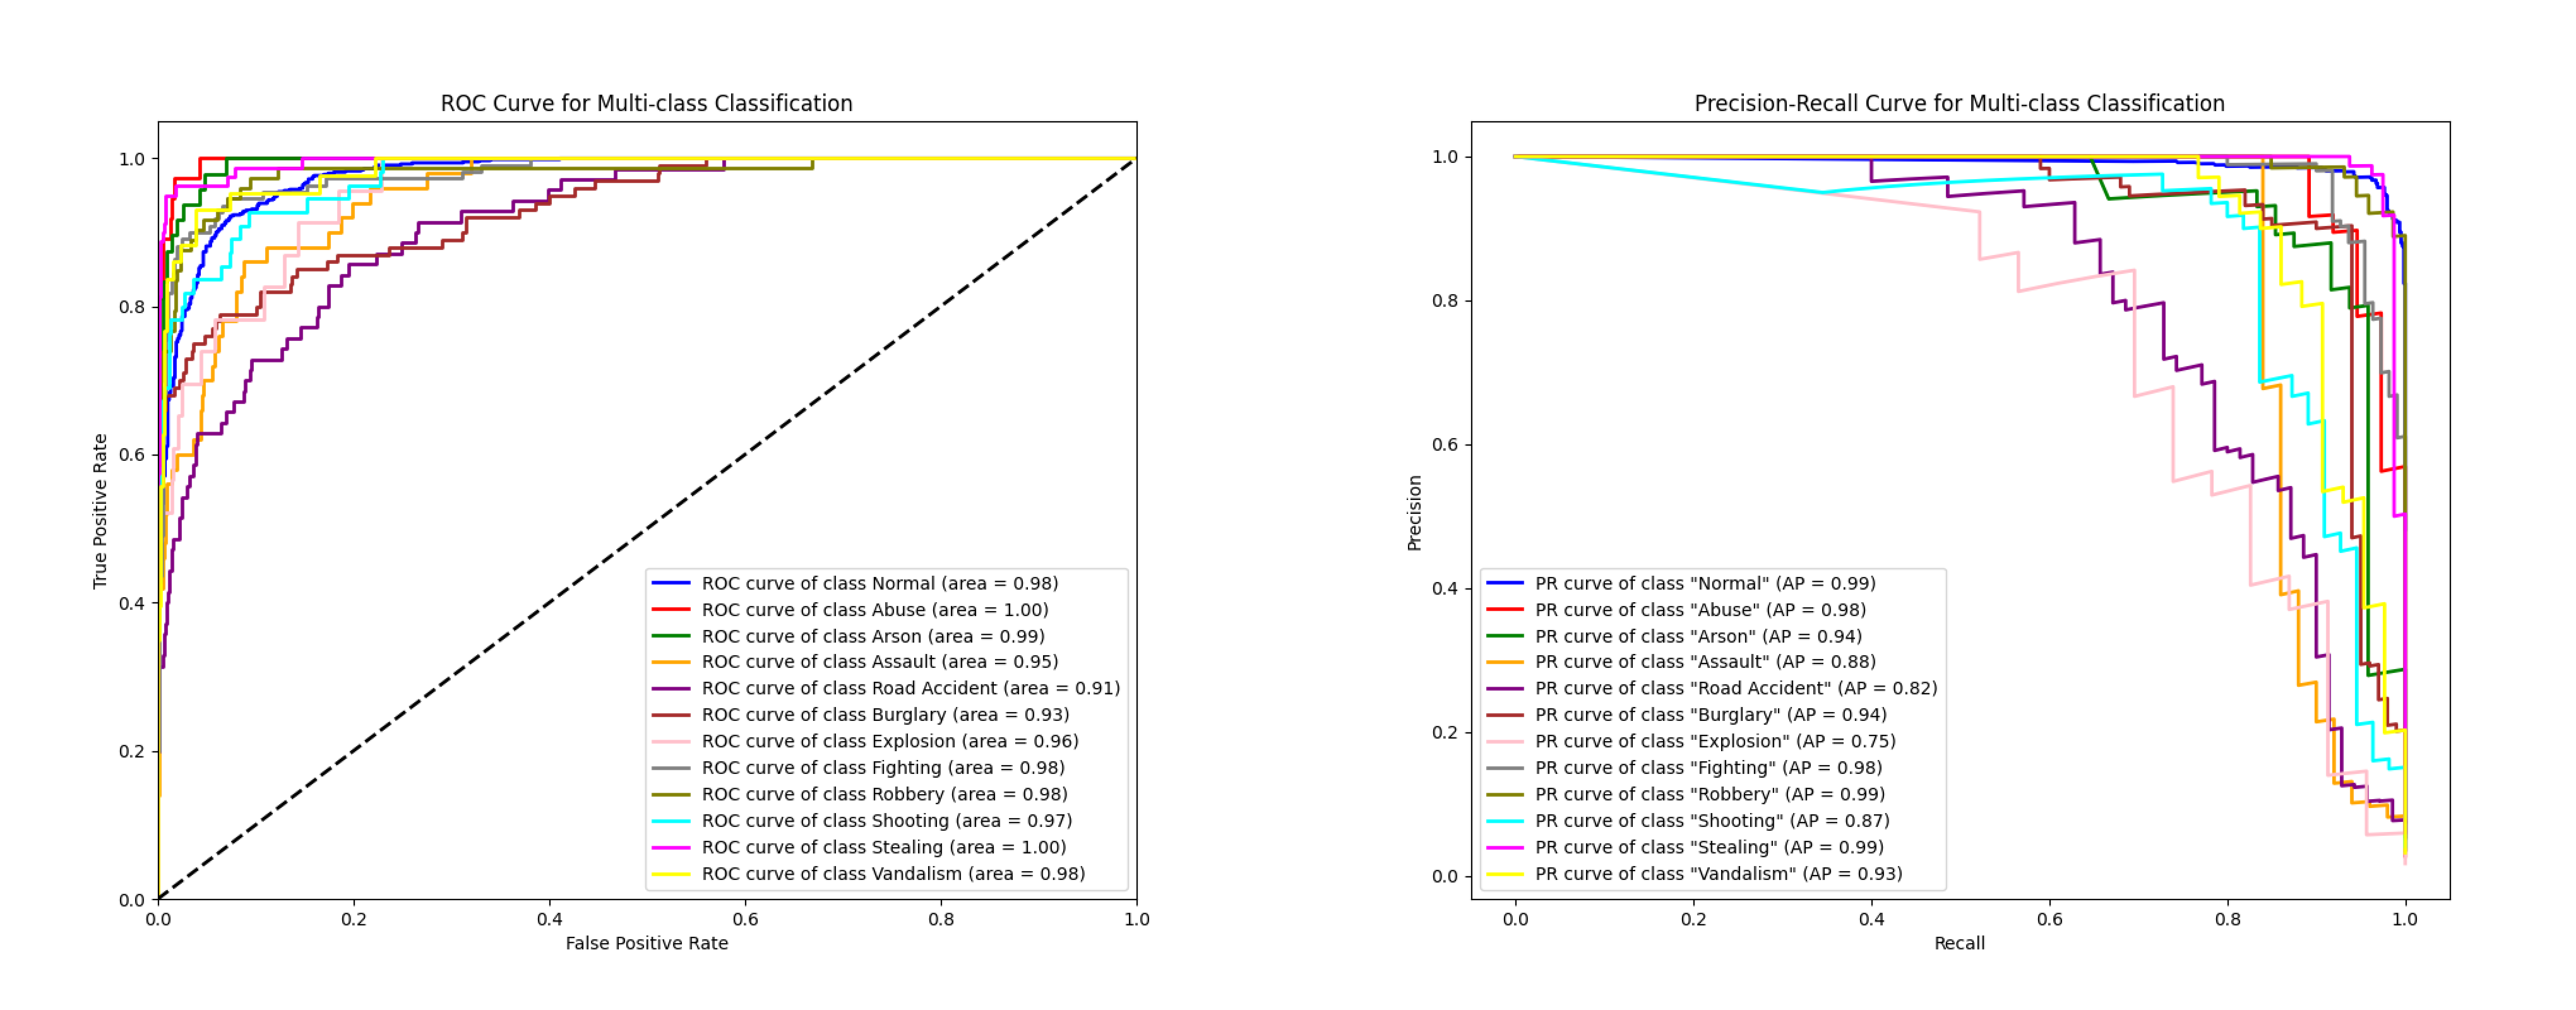
\includegraphics[width=\textwidth]{VAD/FIGURES/rocandpr.png}
\caption{ROC and Precision Recall Curve on Multi-class} \label{Fig 5.}
\end{figure}

\section{Conclusion}
The proposed pipeline has achieved comparable results when compared to the existing models in the landscape of anomaly detection. The model is designed in such a way that the algorithm gets videos representing the true anomalous portion so that the embeddings are created from the input video frames using multi-step feature fusion and contain distinct feature representations, which are then passed down to the recurrent unit for further analysis. Finally, a resultant classification of whether the video is anomalous or not, and if so, which class of anomaly it belongs to in particular. The model has been evaluated using the UCF Crime dataset, where it has proven to be competent enough when compared to the already existing models.


% ---- Bibliography ----
%
% BibTeX users should specify bibliography style 'splncs04'.
% References will then be sorted and formatted in the correct style.
%
% \bibliographystyle{splncs04}
% \bibliography{mybibliography}
%
\begin{thebibliography}{99}

\bibitem{sertis}
Sertis Corp.,
\textit{Title: "Video Anomaly Detection: An Introduction"},
from: Medium,
In: November 30, 2023,
\url{https://sertiscorp.medium.com/video-anomaly-detection-an-introduction-232bf48c9a8d}

\bibitem{sudhakaran}
Sudhakaran, S., Lanz, O.: Learning to detect violent videos using convolutional long short-term memory. In: 2017 14th IEEE International Conference on Advanced Video and Signal Based Surveillance (AVSS), pp. 1--6. IEEE (2017)

\bibitem{petrocchi}
Petrocchi, S., Giorgi, G., Cimino, M.G.: A real-time deep learning approach for real-world video anomaly detection. In: Proceedings of the 16th International Conference on Availability, Reliability and Security, pp. 1--9 (2021)

\bibitem{vosta2022cnn}
Vosta, S., Yow, K.-C.: A cnn-rnn combined structure for real-world violence detection in surveillance cameras. Applied Sciences \textbf{12}(3), 1021 (2022)

\bibitem{islam2021efficient}
Islam, Z., Rukonuzzaman, M., Ahmed, R., Kabir, M.H., Farazi, M.: Efficient two-stream network for violence detection using separable convolutional lstm. In: 2021 International Joint Conference on Neural Networks (IJCNN), pp. 1--8. IEEE (2021)

\bibitem{zhao2022exploiting}
Zhao, M., Liu, Y., Liu, J., Zeng, X.: Exploiting spatial-temporal correlations for video anomaly detection. In: 2022 26th International Conference on Pattern Recognition (ICPR), pp. 1727--1733. IEEE (2022)

\bibitem{zhang2019temporal}
Zhang, J., Qing, L., Miao, J.: Temporal convolutional network with complementary inner bag loss for weakly supervised anomaly detection. In: 2019 IEEE International Conference on Image Processing (ICIP), pp. 4030--4034. IEEE (2019)

\bibitem{qasim2023video}
Qasim, M., Verdu, E.: Video anomaly detection system using deep convolutional and recurrent models. Results in Engineering \textbf{18}, 101026 (2023)

\bibitem{shao2023video}
Shao, W., Xiao, R., Rajapaksha, P., Wang, M., Crespi, N., Luo, Z., Minerva, R.: Video anomaly detection with NTCN-ML: A novel TCN for multi-instance learning. Pattern Recognition \textbf{143}, 109765 (2023)

\bibitem{Multi-contextual}
Lee, J., Nam, W.-J., Lee, S.-W.: Multi-contextual predictions with vision transformer for video anomaly detection. In: 2022 26th International Conference on Pattern Recognition (ICPR), pp. 1012--1018. IEEE (2022)

\bibitem{attention-anomaly}
Deshpande, K., Punn, N.S., Sonbhadra, S.K., Agarwal, S.: Anomaly detection in surveillance videos using transformer based attention model. In: International Conference on Neural Information Processing, pp. 199--211. Springer (2022)

\bibitem{contrastive}
Chang, S., Li, Y., Shen, S., Feng, J., Zhou, Z.: Contrastive attention for video anomaly detection. IEEE Transactions on Multimedia \textbf{24}, 4067--4076 (2021)

\bibitem{Cross-attention}
Kim, H.H., Yu, S., Yuan, S., Tomasi, C.: Cross-attention transformer for video interpolation. In: Proceedings of the Asian Conference on Computer Vision, pp. 320--337 (2022)

\bibitem{Memory-Token}
Li, Y., Song, X., Xu, T., Feng, Z.: Memory-Token Transformer for Unsupervised Video Anomaly Detection. In: 2022 26th International Conference on Pattern Recognition (ICPR), pp. 3325--3332. IEEE (2022)

\bibitem{multi-view}
Li, Q., Yang, R., Xiao, F., Bhanu, B., Zhang, F.: Attention-based anomaly detection in multi-view surveillance videos. Knowledge-Based Systems \textbf{252}, 109348 (2022)

\bibitem{SwinAnomaly}
Bajgoti, A., Gupta, R., Balaji, P., Dwivedi, R., Siwach, M., Gupta, D.: SwinAnomaly: Real-Time Video Anomaly Detection using Video Swin Transformer and SORT. IEEE Access (2023)

\bibitem{TransCNN}
Ullah, W., Hussain, T., Ullah, F.U.M., Lee, M.Y., Baik, S.W.: TransCNN: Hybrid CNN and transformer mechanism for surveillance anomaly detection. Engineering Applications of Artificial Intelligence \textbf{123}, 106173 (2023)

\bibitem{efficientattention}
Ullah, W., Ullah, A., Hussain, T., Khan, Z.A., Baik, S.W.: An Efficient Anomaly Recognition Framework Using an Attention Residual LSTM in Surveillance Videos. \textit{Sensors} \textbf{21}(8), 2811 (2021). \url{http://dx.doi.org/10.3390/s21082811}

\bibitem{stcnet}
Zhao, M., Liu, Y., Li, J., Zeng, X.: Exploiting Spatial-temporal Correlations for Video Anomaly Detection. arXiv. \url{https://arxiv.org/abs/2211.00829} (2022). \doi{10.48550/ARXIV.2211.00829}

\bibitem{prediction}
Li, T., Comer, M.L., Delp, E.J., Desai, S.R., Mathieson, J.L., Foster, R.H., Chan, M.W.: Anomaly Scoring for Prediction-Based Anomaly Detection in Time Series. In: \textit{2020 IEEE Aerospace Conference}, IEEE (2020). \url{http://dx.doi.org/10.1109/AERO47225.2020.9172442}

\bibitem{end2end}
Lai, Y., Liu, R., Han, Y.: Video Anomaly Detection Via Predictive Autoencoder With Gradient-Based Attention. In: \textit{2020 IEEE International Conference on Multimedia and Expo (ICME)}, IEEE (2020). \url{http://dx.doi.org/10.1109/ICME46284.2020.9102894}

\bibitem{cafe}
Yu, G., Wang, S., Cai, Z., Liu, X., Wu, C.: Effective Video Abnormal Event Detection by Learning A Consistency-Aware High-Level Feature Extractor. In: \textit{Proceedings of the 30th ACM International Conference on Multimedia (MM '22)}, ACM (2022). \url{http://dx.doi.org/10.1145/3503161.3547944}

\bibitem{multivit}
Lee, J.-Y., Nam, W.-J., Lee, S.-W.: Multi-Contextual Predictions with Vision Transformer for Video Anomaly Detection. arXiv. \url{https://arxiv.org/abs/2206.08568} (2022). \doi{10.48550/ARXIV.2206.08568}

\bibitem{Yu2022}
Yu, G., Wang, S., Cai, Z., Liu, X., Wu, C.: Effective Video Abnormal Event Detection by Learning A Consistency-Aware High-Level Feature Extractor. In: \textit{Proceedings of the 30th ACM International Conference on Multimedia (MM '22)}, ACM (2022). \url{http://dx.doi.org/10.1145/3503161.3547944}

\bibitem{pkgnet}
Deng, Z., Chen, D., Deng, S.: Prior Knowledge Guided Network for Video Anomaly Detection. arXiv. \url{https://arxiv.org/abs/2309.01682} (2023). \doi{10.48550/ARXIV.2309.01682}

\bibitem{state}
Wang, Y., Qin, C., Bai, Y., Xu, Y., Ma, X., Fu, Y.: Making Reconstruction-based Method Great Again for Video Anomaly Detection. arXiv. \url{https://arxiv.org/abs/2301.12048} (2023). \doi{10.48550/ARXIV.2301.12048}

\bibitem{ma}
Zhu, Y., Newsam, S.: Motion-Aware Feature for Improved Video Anomaly Detection. arXiv. \url{https://arxiv.org/abs/1907.10211} (2019). \doi{10.48550/ARXIV.1907.10211}

\bibitem{he2015deep}
He, K., Zhang, X., Ren, S., Sun, J.: Deep Residual Learning for Image Recognition. arXiv:1512.03385 (2015).

\bibitem{lei2018simple}
Lei, T., Zhang, Y., Wang, S. I., Dai, H., Artzi, Y.: Simple Recurrent Units for Highly Parallelizable Recurrence. (2018). arXiv:1709.02755 [cs.CL]

\bibitem{lei2021attention}
Lei, T.: When Attention Meets Fast Recurrence: Training Language Models with Reduced Compute. arXiv:2102.12459 [cs.CL] (2021)

\bibitem{zhou2023batchnorm}
Yixuan Zhou, Yi Qu, Xing Xu, Fumin Shen, Jingkuan Song, Hengtao Shen. "BatchNorm-based Weakly Supervised Video Anomaly Detection." arXiv preprint arXiv:2311.15367 (2023).

\bibitem{challenges}
Ren, J., Xia, F., Liu, Y., \& Lee, I. (2021). "Deep video anomaly detection: Opportunities and challenges." In 2021 International Conference on Data Mining Workshops (ICDMW) (pp. 959-966). IEEE.

\bibitem{gan2023contrastive}
Kian Yu Gan, Yu Tong Cheng, Hung-Khoon Tan, Hui-Fuang Ng, Maylor Karhang Leung, Joon Huang Chuah. "Contrastive-regularized U-Net for video anomaly detection." IEEE Access (2023).

\bibitem{dubey20193d}
Shikha Dubey, Abhijeet Boragule, Moongu Jeon. "3D ResNet with ranking loss function for abnormal activity detection in videos." 2019 international conference on control, automation and information sciences (ICCAIS), IEEE (2019).

\bibitem{wu2022self}
Jhih-Ciang Wu, He-Yen Hsieh, Ding-Jie Chen, Chiou-Shann Fuh, Tyng-Luh Liu. "Self-supervised sparse representation for video anomaly detection." European Conference on Computer Vision, Springer (2022).


\end{thebibliography}

\end{document}
